\documentclass[UTF8]{beamer}

\usetheme{Madrid}
\usecolortheme{seagull}

\usepackage[english]{babel}
\usepackage{ctex}
\usepackage{algorithm,algorithmicx,algpseudocode}
\usepackage{tabularx}
\usepackage{graphicx}
\graphicspath{ {img/} }

\begin{document}

\title{Hush up! 题目讨论}
\author{CyanD1317 / Tommyr7 / wangyurzee}
\frame{\titlepage}


\begin{frame}{Problem 1. STUMBLER}

给定一个简化的物件组成的 osu! 谱面,从原点出发等概率选择一个方向发出一条射线,%
求有且仅有一个物件在射线上的概率。

\begin{itemize}
    \item $N_\mathrm{C}, N_\mathrm{S} \leq 50\,000$
    \item 精度 $10^{-6}$
\end{itemize}

\end{frame}

\begin{frame}{Observations \& Lemmata}

\begin{itemize}
\item
    将 $-\pi$ 和 $+\pi$ 看作首尾相接,那么一个物件影响的角度范围是连续的,%
    且该范围不会大于等于 $\pi$。
    \begin{itemize}
        \pause
        \item Formally:如果射线 $OA$ 与射线 $OB$ 都与物体 $U$ 有公共点,
            那么在劣角 $AOB$ 内的任意一条射线 $OC$ 都与物体 $U$ 有公共点。
        \pause
        \item 显然成立。
    \end{itemize}
\pause
\item
    在前两个子任务的限制下,物件影响的角度范围没有重叠部分。
    \begin{itemize}
        \pause
        \item 计算出每个物件的影响的范围大小,相加即为答案。
    \end{itemize}
\end{itemize}

\end{frame}

\begin{frame}{Algorithm 1}

子任务 1:只有圆形物件,物件影响的角度范围没有重叠部分。

\begin{figure}[h]\centering
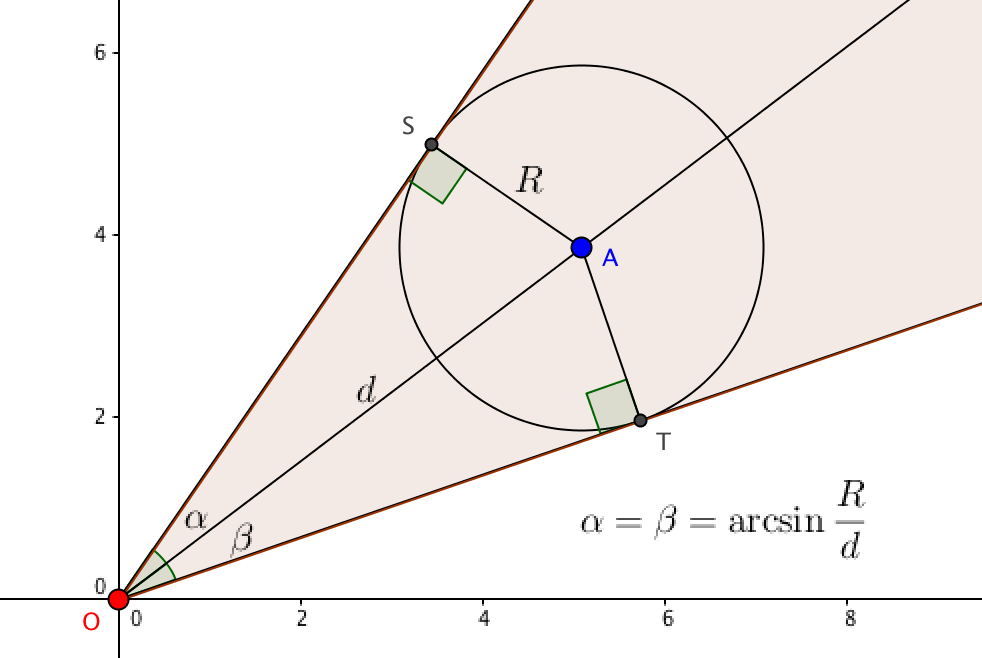
\includegraphics[scale=0.48]{a1.png}
\end{figure}

\end{frame}

\begin{frame}{Algorithm 2}

子任务 2:有滑条物件,物件影响的角度范围没有重叠部分。

\begin{figure}[h]\centering
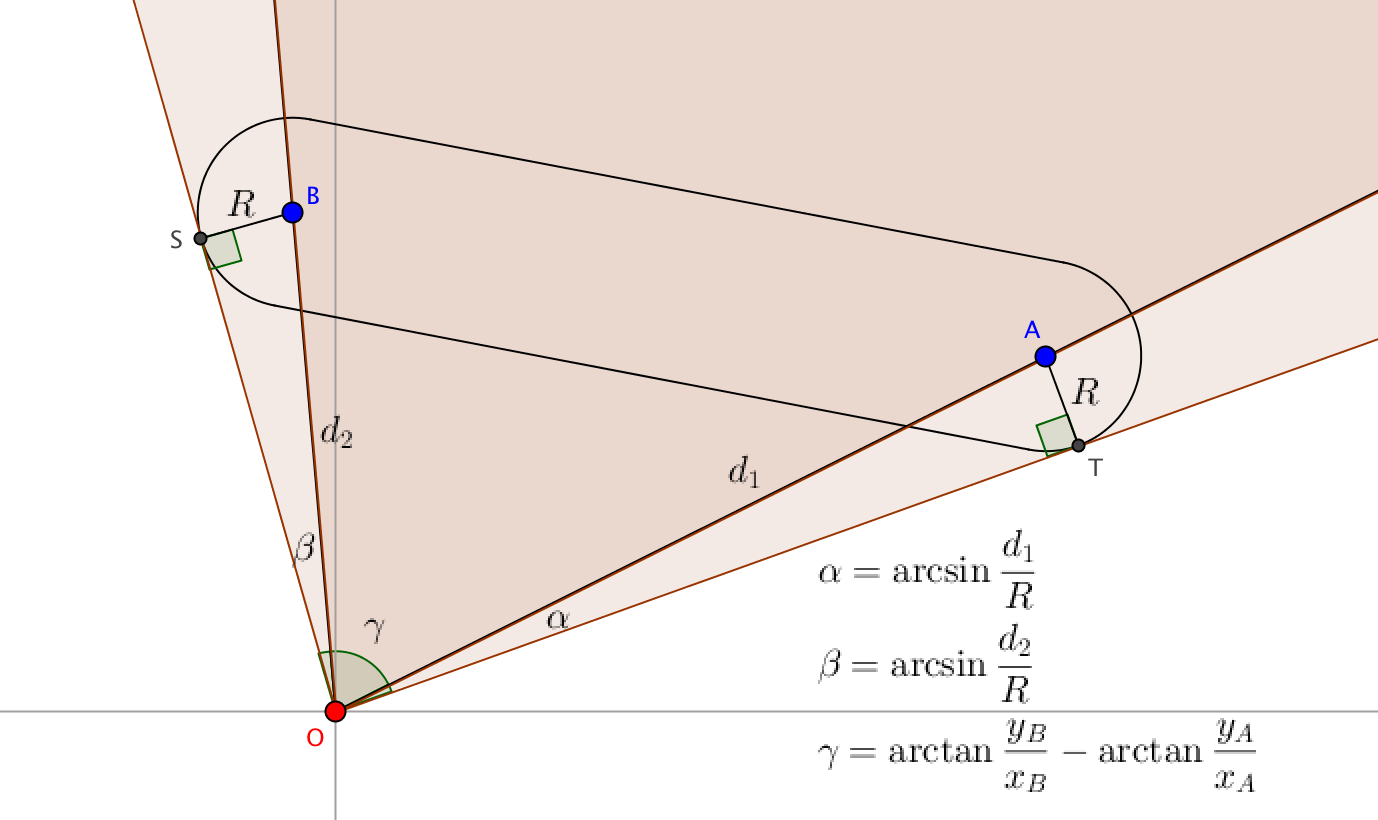
\includegraphics[scale=0.4]{a2.png}
\end{figure}

\end{frame}

\begin{frame}{Algorithm 2}

特殊情况:与上一种取 max

\begin{figure}[h]\centering
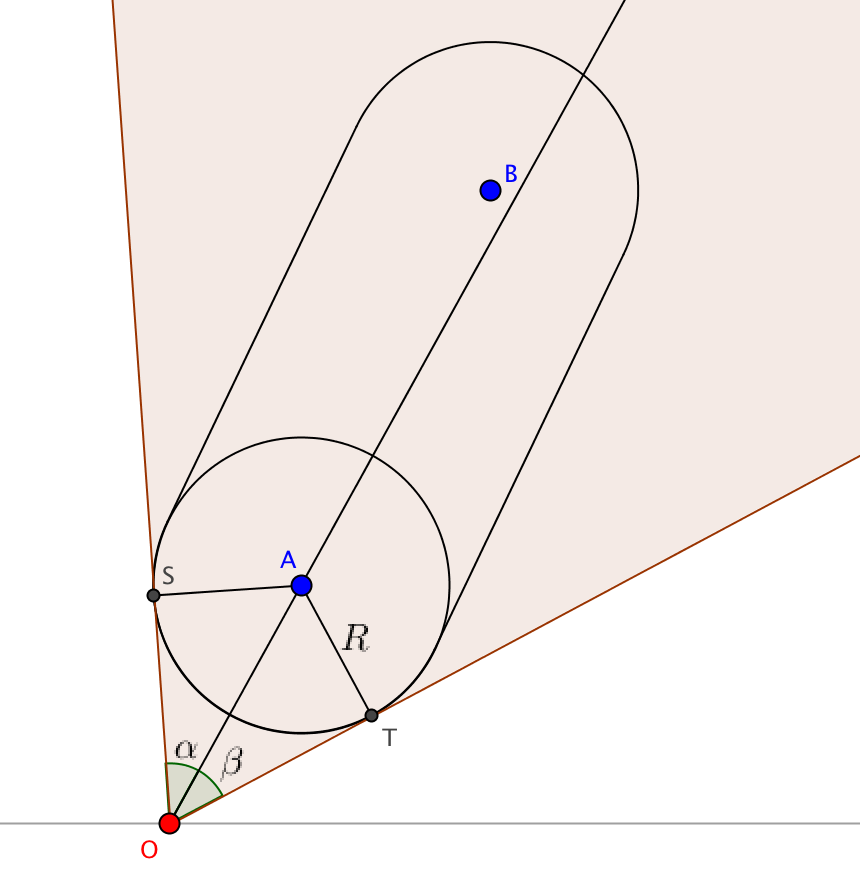
\includegraphics[scale=0.4]{a3.png}
\end{figure}

\end{frame}

\begin{frame}{Algorithm 3}

子任务 3:$N_\mathrm{C}, N_\mathrm{S} \leq 1\,000$ \newline

不会做,输出 QAQ

\begin{figure}[h]\centering

\includegraphics[scale=0.5]{xx.png}
\end{figure}

\end{frame}

\begin{frame}{Algorithm 4}

子任务 4:存在一条从原点出发的射线与每一个打击物件都有公共点。

\begin{figure}[h]\centering
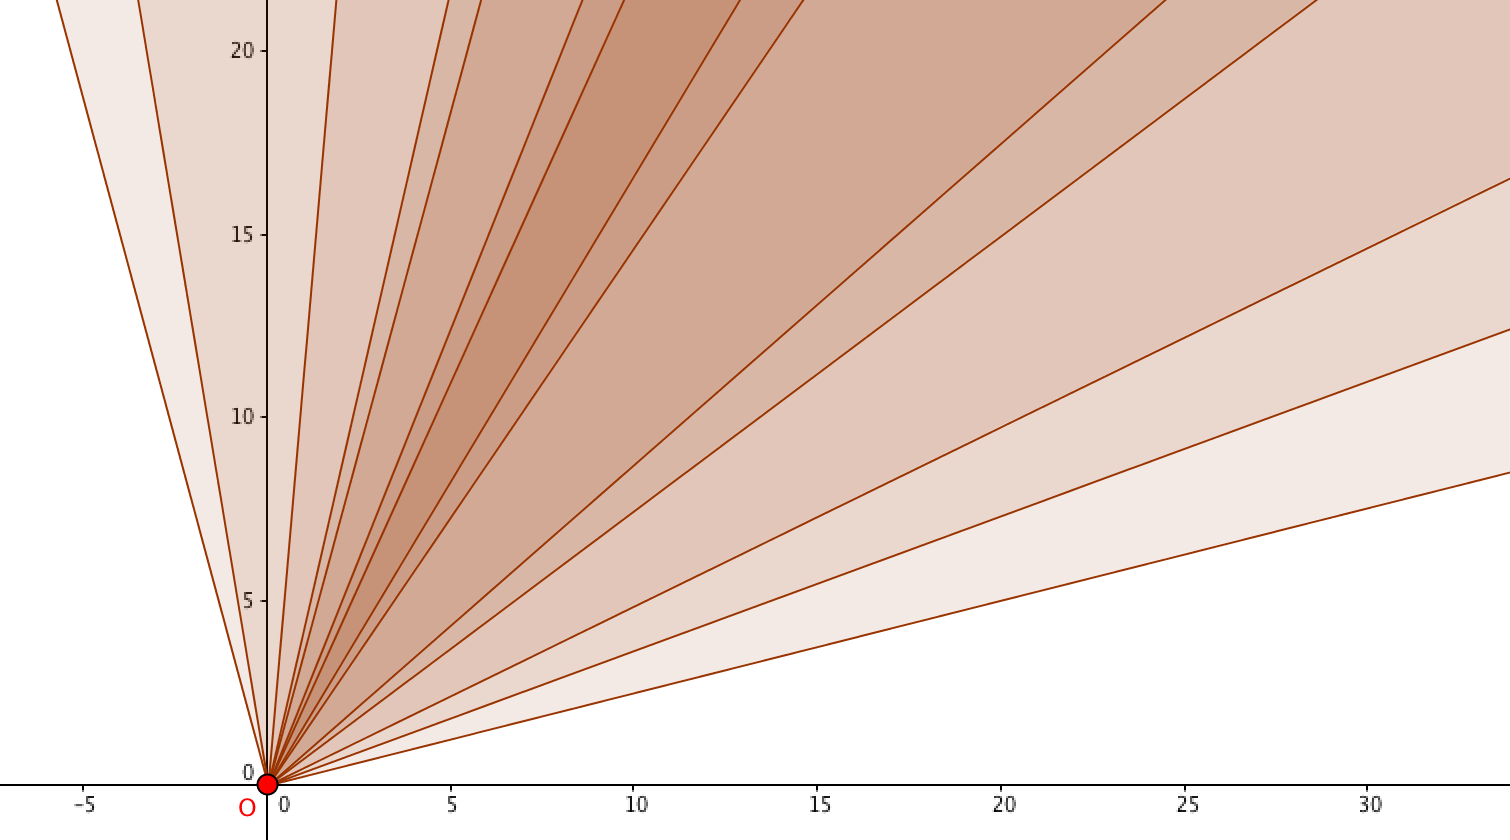
\includegraphics[scale=0.4]{a4.png}
\end{figure}



\end{frame}

\begin{frame}{Algorithm 5}

子任务 3:$N_\mathrm{C}, N_\mathrm{S} \leq 1\,000$ \newline

\begin{itemize}
    \pause \item 按照上述方法计算出每个物件影响角度的区间,记录端点(线?←\_←)并排序
    \pause \item 跨过 $\pm \pi$ 的位置拆分为两个区间
    \pause \item 枚举两个相邻端点,检查它们所夹区间是否被恰好一个物件覆盖
    \pause \item 排序 $O(N^2)$,枚举共 $O(N)$ 个区间,检查一次 $O(N)$
    \item 总时间复杂度 $O(N^2)$
\end{itemize}

\end{frame}

\begin{frame}{Algorithm 6}

我会快速排序!
\includegraphics[scale=0.666]{yy.png} \newline\newline

\pause $O(N \log N) + O(N^2) = O(N^2)$

\end{frame}

\begin{frame}{Algorithm 7}

“枚举两个相邻端点,检查它们所夹区间是否被恰好一个物件覆盖”\newline\newline

优化?

\end{frame}

\begin{frame}{Algorithm 7}

\begin{figure}[h]\centering
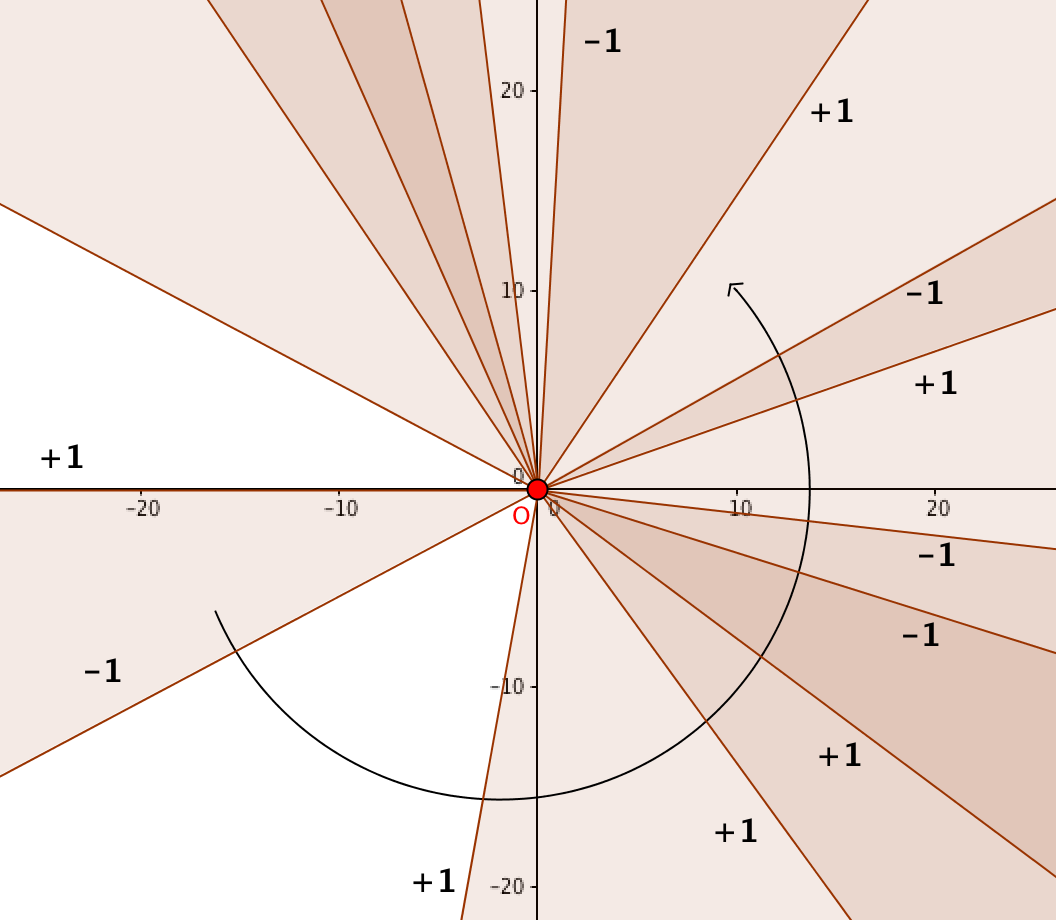
\includegraphics[scale=0.333]{a5.png}
\end{figure}

把区间转化成“事件”,对事件排序并依次处理,记录上个事件的位置与%
当前覆盖层数,判断层数 = 1 时增加答案。(常用 trick)

时间复杂度 $O(N \log N) + O(N) = O(N \log N)$

\end{frame}


\begin{frame}{Problem 2. OBSESSED}

给定一个序列,每个位置上为“空”、“面”音符与“边”音符中的一种。

进行下列操作:
\begin{itemize}
    \item 放置“面”或“边”音符;
    \item 询问一段连续区间内最近一对相同音符(“面”或“边”)之间的最小距离。
\end{itemize}

$N, M \leq 300\,000$

\end{frame}

\begin{frame}{Algorithm 1}

子任务 1、2:$N \cdot M \leq 600\,000$

直接模拟即可。注意反转操作的判定\newline\newline

\begin{algorithm}[H]
\begin{algorithmic}[1]
    \If {$A[i] = \mathrm{DON}$}
        \State $A[i] \gets \mathrm{KAT}$
    \Else
        \State $A[i] \gets \mathrm{DON}$
    \EndIf
\end{algorithmic}
\caption{ 
\includegraphics[scale=0.2]{zz.jpg}}
\label{alg:seq}
\end{algorithm}

\end{frame}

\begin{frame}{Algorithm 2}

子任务 3:没有“边”音符和反转操作,放置音符的位置严格单调递增

\begin{figure}[h]\centering
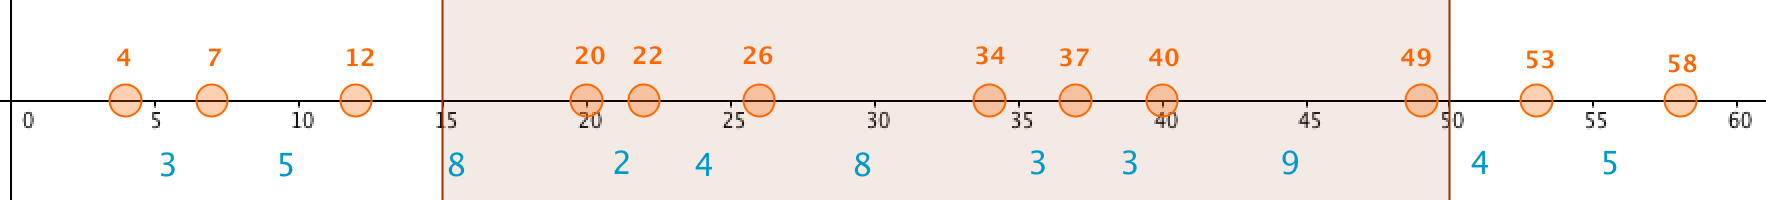
\includegraphics[scale=0.4]{b1.png}
\end{figure}

\begin{itemize}
    \pause \item 找出对应的音符范围:二分查找,$O(\log N)$
    \pause \item 在范围内查询最小值:Range Minimum Query,线段树 $O(\log N)$
\end{itemize}

\end{frame}

\begin{frame}{Algorithm 3}

子任务 4:存在两种音符,没有反转操作 \newline\newline

看着好像线段树的样子

\end{frame}

\begin{frame}{Algorithm 3}

对于一个线段树的节点而言,需要考虑的情况有以下三种:
\begin{itemize}
    \item 完全在左子节点的区间中;
    \item 完全在右子节点的区间中;
    \item 跨越左右子节点区间的交界处。
\end{itemize}

\pause
为了实现两段区间信息的合并,需要在每个节点上记录……?

\pause
\textbf{最左/最右的鼓面/鼓边音符}共 4 条信息。\\
另外自己内部的最优答案也要记录。

\end{frame}

\begin{frame}{Updating Segment Tree Nodes}

\begin{algorithm}[H]
\begin{algorithmic}[1]
    \Function {Update}{$node$}
        \If {$node.lch = -1$} \State \Return \EndIf
        \State $node.lmost\_don = \min(node.lch.lmost\_don, node.rch.lmost\_don)$
        \State $node.rmost\_don = \min(node.lch.rmost\_don, node.rch.rmost\_don)$
        \State $node.lmost\_kat = \min(node.lch.lmost\_don, node.rch.lmost\_kat)$
        \State $node.rmost\_kat = \min(node.lch.rmost\_don, node.rch.rmost\_kat)$
        \State $node.ans = \min(node.lch.ans, node.rch.ans)$
        \State $node.ans = \min(node.ans, node.rch.lmost\_don - node.lch.rmost\_don)$
        \State $node.ans = \min(node.ans, node.rch.lmost\_kat - node.lch.rmost\_kat)$
    \EndFunction
\end{algorithmic}
\caption{}
\label{alg:seq}
\end{algorithm}

\end{frame}

\begin{frame}{Algorithm 3}

时间复杂度 $O(M \log N)$。

\end{frame}

\begin{frame}{Algorithm 4}

子任务 5:存在两种音符和反转操作 \newline\newline

看着好像线段树的样子

\begin{figure}[h]\centering

\includegraphics[scale=0.5]{xx.png}
\end{figure}

\end{frame}

\begin{frame}{Algorithm 4}

\textbf{延迟标记/懒标记}

每个节点除了记录上述信息外,额外记录一个布尔变量 $tag$%
表示该节点下所有的音符是否被 Invert

维持 $lmost, rmost$ 与 $tag$ 同步更新(即 $lmost, rmost$%
记录的是 $tag$ 生效后的值)。访问到一个节点时,若该节点的%
$tag$ 为真,那么将 $tag$ 下传到左右子节点并更新各自信息。

\end{frame}

\begin{frame}{Handling Lazy Tag Propagation}

\begin{algorithm}[H]
\begin{algorithmic}[1]
    \Function {PushDown}{$node$}
        \If {$node.lch = -1$ \textbf{or} $node.tag = $ \textbf{false}}
            \State \Return
        \EndIf
        \State $node.tag \gets$ \textbf{false}
        \State $node.lch.tag \gets$ \textbf{not} $node.lch.tag$
        \State $node.rch.tag \gets$ \textbf{not} $node.rch.tag$
        \State \Call{Swap}{$node.lch.lmost\_don, node.lch.lmost\_kat$}
        \State \Call{Swap}{$node.lch.rmost\_don, node.lch.rmost\_kat$}
        \State \Call{Swap}{$node.rch.lmost\_don, node.rch.lmost\_kat$}
        \State \Call{Swap}{$node.rch.rmost\_don, node.rch.rmost\_kat$}
    \EndFunction
\end{algorithmic}
\caption{}
\label{alg:seq}
\end{algorithm}

\end{frame}

\begin{frame}{Algorithm 4}

时间复杂度 $O(M \log N)$。

具体细节参见参考程序或者两段伪代码。

\end{frame}

\end{document}

